\graphicspath{{./experiment/}}

\chapter{Experiment}
% {{{
\label{cha:experiment}

The position data to be compressed in our water compression system is floating
point data. To facilitate compression, the floating point data is converted to
integer values through quantisation. An appropriate number of bits, the range
of integer values, to use will need to be decided. Fewer bits used will result
in higher compression, but more quantisation error will be incurred; while more
bits used will result in lower compression, but the data is stored more
accurately.

To determine the appropriate level of quantisation, an experiment was conducted
to test the perceptually visible effects of quantisation. More simply stated:
how noticable are the effects of quantisation? This will help determine the
appropriate level of quantisation; using the least number of bits, while
maintaining visual similarity to the original data.

The rest of this chapter details various aspects of the experiment.

\section{Introduction}
% {{{
\label{sec:experiment_introduction}

The participants in the experiment were required to rate the difference between
the original unquantised data, and the quantised data. The participants used a
scale of 1 to 7 to rate the difference. Two different visualisation techniques,
and four different quantisation levels were tested. The experiment procedure is
detailed in Section \ref{sec:experiment_procedure}.

Figures \ref{fig:experiment_ballstick4680} and
\ref{fig:experiment_metaballs4680} shows the different quantisation levels for
the ball and stick, and metaballs visualisation techniques respectively. The
original unquantised data is on the left, with the four different quantisation
levels; 10 and 8 bit quantisation at the top, 6 and 4 bit quantisation at the
bottom.

\begin{figure}[h!]
  \begin{center}
    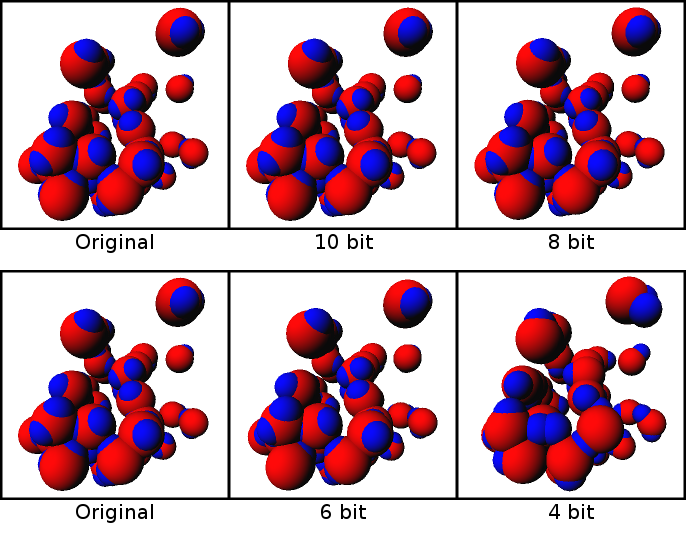
\includegraphics[width=120mm]{ballstick4680}
  \end{center}
  \caption{Ball and stick visualisation showing the different quantisation
  levels}
  \label{fig:experiment_ballstick4680}
\end{figure}

\begin{figure}[h!]
  \begin{center}
    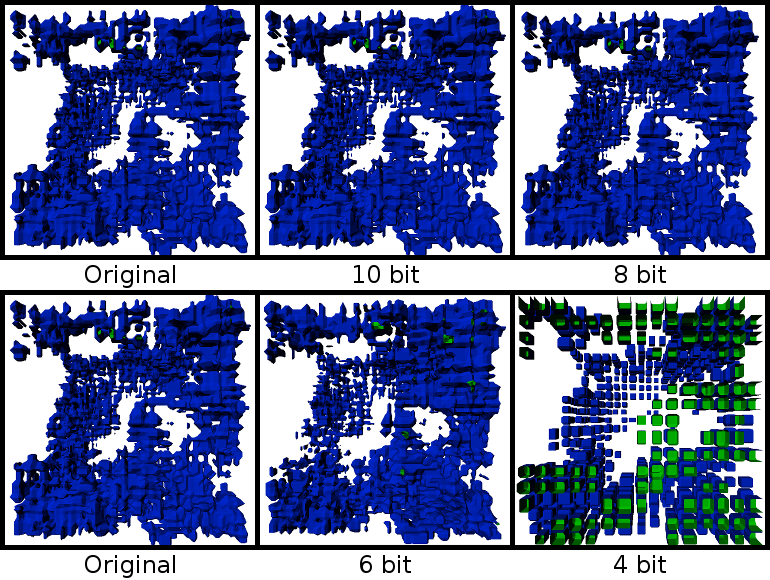
\includegraphics[width=120mm]{metaballs4680}
  \end{center}
  \caption{Metaballs visualisation showing the different quantisation
  levels}
  \label{fig:experiment_metaballs4680}
\end{figure}

% }}}

\section{Venue and equipment}
% {{{
\label{sec:experiment_venue}

The participants took part in the experiment one at a time within a closed
room. They watched the data on a monitor, which was connected to a laptop. The
laptop was used to load and display the data. The same laptop was used for all
the experiments:
\begin{itemize}
  \item Processor: Intel Core 2 Duo Processor T6570 2.1GHz
  \item Memory: 2GB DDR2
  \item GPU: Mobile Intel Graphics Media Accelerator X4500 HD
\end{itemize}

% }}}

\section{Participants}
% {{{
\label{sec:experiment_participants}

All the partipants were students from the University of Cape Town. Half of the
participants were Science students, with the remaining half consisting of
mostly Commerce and Humanities students.

The only requirement for a participant to take part in the experiment is that
they are not visually impaired. All that is needed is that they are able to
watch and compare two different sets of data (molecular visualisations).

A total of 30 participants took part in the experiment. Most of the experiments
were completed in the first three days (25 of the planned 30), while the
remaining experiments completed over three more days.

% }}}

\section{Variables}
% {{{
\label{sec:experiment_variables}

The variables of the experiment are the four different quantisation levels, and
the two different visualiation techniques.

The four quantisation levels tested were:
\begin{itemize}
  \item 4 bit quantisation
  \item 6 bit quantisation
  \item 8 bit quantisation
  \item 10 bit quantisation
\end{itemize}

10 bit quantisation was chosen as the upper quantisation level to test because
beyond 10 bits, the quantisation effects are too minimal to be noticeable. Even
at 10 bit quantisation, the differences are miniscule (see Figure
\ref{fig:experiment_ballstick4680}).

The two visualisation techniques were:
\begin{itemize}
  \item Ball and stick view
  \item Metaballs view
\end{itemize}

At the time of the experiment, there were four datasets available, all of which
were used and randomly selected for the participants.

% }}}

\section{Procedure}
% {{{
\label{sec:experiment_procedure}

\begin{enumerate}

  \item The subject will be given a piece of paper explaining the experiment
  and what they are to do.

  \item A random dataset is selected for the participant.

  \item The original unquantised data will be loaded and the subject will be
  allowed to explore and view it.

  \item Thereafter, two different quantised data will be loaded for the subject
  to see.

  \item The original data will the loaded again to remind the participant what
  the original data looked like.

  \item A final two more quantised data will be loaded.

  \item The quantisation levels will be chosen in a random order.

  \item After showing each quantised data, the subject will be asked to compare
  it with the original data, indicating on a scale of 1 to 7, how noticeable the
  differences are: 1 being ``Not noticeable'' and 7 being ``Very obvious''.

  \item This procedure will be repeated for a total of 2 visualisation
  techniques, with 2 different datasets each.

  \item The order of visualisation techniques shown will be the same: ball and
  stick, then metaballs.

\end{enumerate}

On average, the participants took 25 minutes to complete the experiment. The
duration of the experiment varied due to the different datasets. Not all the
datasets were of equal size or length, some datasets required more time to play
from start to finish.

After conducting a pilot experiment, it was decided that the participants
should not be able to rotate and explore the data. Rotating the view makes the
data look very different and the participants may become lost and disoriented.
This could invalidate the results of the experiment as the participants will
not be able to accurately compare the unquantised and quantised data.

% }}}

\section{Summary}
% {{{
\label{sec:experiment_summary}

The experiment used the: ball and stick, and metaballs visualisation
techniques; with 4, 6, 8 and 10 bit quantisation levels. A total of 30
participants took part in the experiment, each of which viewed two different
datasets. There were four datasets used in the experiment, thus, each dataset
was viewed by 15 participants.

Over the four datasets, a total of 60 ratings per quantisation level was
recorded. The results from the experiment is presented and analysed in Chapter
\ref{cha:results}.

% }}}

% }}}

